\chapter{System do klasyfikacji elementów morometrycznych krwi}
\label{cha:system_do_klasyfikacji_elementow_morfologicznych}

\section{Przygotowanie bazy danych}
\label{przygotowanie_danych}

Baza danych zawiera 12500 zdjęć krwinek białych w formacie JPEG wykonanych pod mikroskopem. Pogrupowane są w cztery foldery według przynależności do klas, każdy po około 3000 ramek. Uwzględnione typy krwnek to neutrofil, eozynofil, limfocyt, monocyt. Zbiór został stworzony z 410 obrazów przez operację powiększania zbioru (ang. \textit{data augmentation}) \cite{database_kaggle}.

{\parindent0pt % disables indentation for all the text between { and }
Ramki wczytane bezpośrednio z bazy źródłowej do programu są w formacie RGB. Piksele oryginalnych obrazów mogą przyjmować wartości z zakresu od 0-255. Dla lepszego działania sieci neuronowej zaleca się normalizację wartości pikseli do małego zakresu, najlepiej 0-1 oraz ustandaryzowanie tak, aby można było traktować dane wejściowe jako rozkład Gaussa o średniej 0 i odchyleniu standadowym 1 (\ref{equ:standarisation}), \cite{standarisation}.

\begin{equation}
z =  \frac{x - \mu}{\sigma} 
\label{equ:standarisation}
\end{equation}
gdzie,
\begin{eqwhere}[2cm]
	\item[$x$] oryginalna wartość piksela,
	\item[$\mu$] średnia z wartości pikseli w ramce,
	\item[$\sigma$] odchylenie standardowe wartości pikseli w ramce,
	\item[$z$] wartość piksela po ustandaryzowaniu.
\end{eqwhere}
}

\subsection{Zastosowanie metody augmentacji danych}
W przypadku małych zbiorów danych, rozumianych jako zbiór liczący kilka tysięcy elementów często stosowaną praktyką jest poszerzanie zboru danych. Ma ona na celu bezpośrednio powiększenie ilości danych wprowadzanych do modelu, a pośrednio polepszenie rezultatów klasyfikacji. Jednym z korzystnych efektów tego działania jest redukcja zjawiska nadmiernego dopasowania (\textit{ang. overfiting}). Objawia się ona zmniejszeniem różnicy między błędem zbioru, na którym się trenuje model a błędem zbioru, na którym model jest testowany. Szczególnie dużą poprawę w tym aspekcie obserwuje się właśnie dla sieci typu CNN \cite{Wong2016UnderstandingDA}.

{\parindent0pt % disables indentation for all the text between { and }
Jednym ze sposobów transformacji jest elastczna deformacja w przestrzenii danych (\textit{ang. data-space elastic deformation}). Obrazy w oryginalnym zbiorze danych zostają poddane losowym transformacjom, z założeniem, że zachowane zostają informacje o przynależności do danej klasy. Daje najlepsze rezultaty w porównaniu do poszerzania w przestrzenii cech (\textit{ang. feature-space augmentation}) \cite{Wong2016UnderstandingDA}. Definiuje ona znormalizowany obszar losowego przemieszczenia \(u(x,y)\), który dla każdego piksela w obrazie \((x,y)\) definiuje wektor przemieszczenia \(R_w\) (\ref{equ:augmentation}), \cite{Wong2016UnderstandingDA}:

\begin{equation}
R_w = R_0 + \alpha u
\label{equ:augmentation}
\end{equation}
gdzie,
\begin{eqwhere}[2cm]
	\item[$R_w$] lokalizacja piksela w obrazie wyjściowym,
	\item[$R_0$] lokalizacja piksela w oryginalnym obrazie,
	\item[$\alpha$] wielkość przesunięcia w pikselach.
\end{eqwhere}
%Odległość półpauzy od lewego marginesu należy dobrać pod kątem najdłuższego symbolu (bądź listy symboli) poprzez odpowiednie ustawienie parametru tego środowiska (domyślnie: 2 cm).

Nie jest wskazane używanie zbioru powiększonego z użyciem dużych transformacji. Dla bazy MNIST przesunięcia \( \alpha \geq 8 \)  pikseli skutkuje w pewnej części przypadków utratą informacje o przynależności do danej klasy. Jest to definiowane jako brak zdolności do rozpoznania i zaklasfikowania danej ramki przez człowieka \cite{Wong2016UnderstandingDA}.

W przypadku rozpoznawania typów komórek augmentacja z zastosowaną zmianą skali może skutkować pogorszeniem dokładności klasyfikacji, gdyż na każdy rodzaj komórki ma swoją typową wielkość. Skorzystanie z tej cechy do nauczenia się rozpoznawania elementów z pewnością podnosi poziom precyzji działania algorytmu. Zaburzenie tej cechy przez manipulację skalą zdjęcia będzie skutkować utraceniem tej informacji. Zbiór danych zostanie powiększony, jednak stanie się to kosztem utraty pewnych pomocnych danych.

Baza danych użyta w pracy oryginalnie zawiera obrazy, będące wynikiem operacji powiększania zbioru. Oryginalna baza danych zawierała 410 obrazów krwinek białych. W wyniku powięszania zbiou powstała baza wkorzystywana w niniejszym projekcie. Z tego powodu nie jest wskazane dodatkowe przepowadzanie powiększania. Sumarcznie, użyta baza zawiera 12444 obrazy krwinek białych z czterech rozpatrywanych kategorii.
}

\subsection{Podział na podzbiory}

W celu wykorzystania danych do stworzenia sieci należy je podzielić na podzbiory: uczący - służący do wytrenowania sieci, walidacyjny - służący do nastrojenia sieci oraz testowy - użyty tylko raz na samym końcu gdy klasyfikator jest gotowy w celu sprawdzenia skuteczności sieci na nowych danych.

{\parindent0pt
Sposób podziału bazy danych na zbiory ma znaczący wpływ na jakość klasyfikatora, jaki można uzyskać. W przpadku przeznaczenia dużej ilości danych do treningu łatwiejsze będzie uzyskanie dobrej skuteczności na danych teningowych. Jednak nie da to pewności czy sieć zadziała poprawnie dla nowych danych, gdyż zbiory walidacyjny i testowy będą ograniczone. W sytuacji odwrotnej, przy użyciu dużej ilości danych do strojenia i testów sieć może nie nauczyć się odpowiedniej ilości różnorodnych wzorców, gdyż zbiór treningowy został ograniczony.

Początkowym podział bazy na zbiory został zrobion zgodnie z podejściem zastosowanym w rozdziale \ref{sec:section_kaggle_1}. Dzięki temu uzyskane wyniki będą mogły być porównywane.
}

\section{Zaproponowana struktura sieci neuronowej}
%narzędzie do rysowania sieci: http://alexlenail.me/NN-SVG/LeNet.html
%ResNet - spróbować wpiąć do mojej sprzężenie tak jak tutaj: https://medium.com/analytics-vidhya/cnns-architectures-lenet-alexnet-vgg-googlenet-resnet-and-more-666091488df5
Struktura sieci neuronowej bazuje na wybranych cechach zaczerpiętych z architektur VGGNet, U-Net oraz ResNet. W kolejnych podrozdziałach zostały opisane poszczególne modele, których charakterystyczne wlasności wykorzystano w końcowym rozwiązaniu.

\subsection{Cechy architektury zaczerpnięte z modelu VGGNet.}

VGGNet jest to architektura sieci kowolucyjnej opublikowanej przez Visual Geometry Group na Universitecie Oksfordzkim w 2014 roku \cite{VGG16_info}. Wytrenowana na 1.3 milionach obrazów treningowych dzielących się na 1000 klas uzyskała 92,7\% skuteczności na zbiorze testowym \cite{deep_learning_w_keras} \cite{VGG16_article_online}. Charakteryzuje się jednolitą budową i składa się jedynie z warstw konwolucyjnych przekładanych co dwie lub trzy warstwy redukcją maksymalizującą oraz trzech warstw gęsto połączonych, umieszczonych na końcu modelu (Rys. \ref{fig:vgg_16_stucture}). Najczęściej w literaturze występuje w wersjach z 16 (VGG16) i 19 (VGG19) warstwami konwolucyjnymi. 

\begin{figure}[h]
	\centering
	\centering
		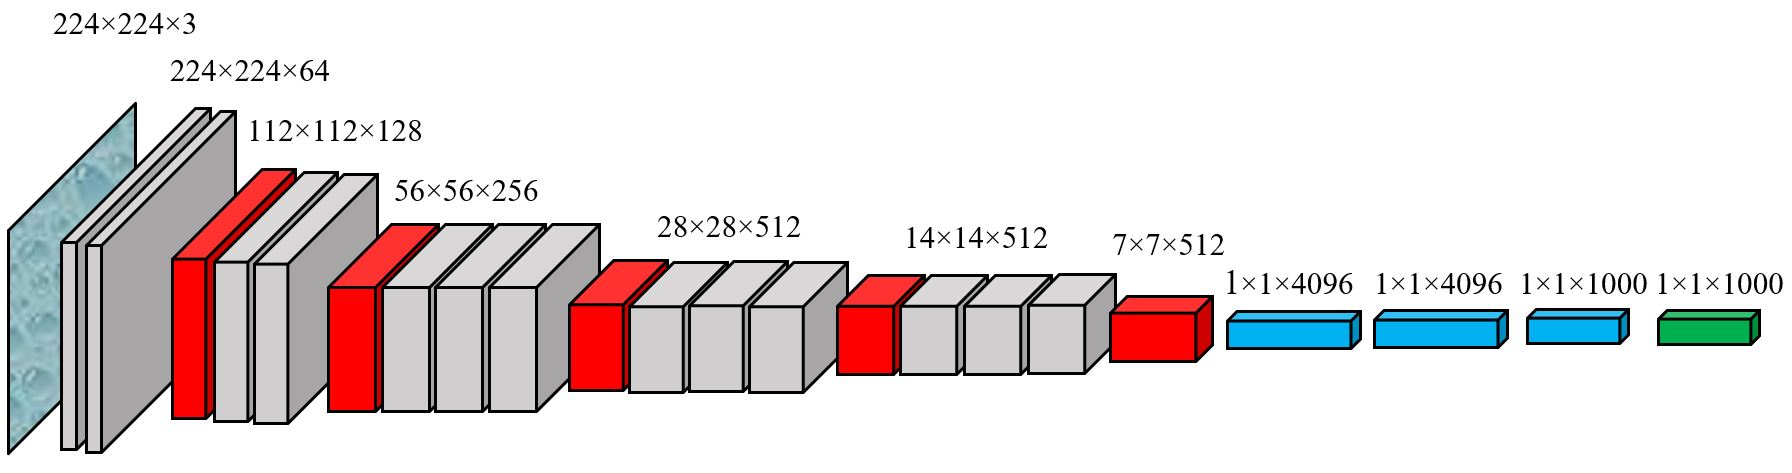
\includegraphics[scale=0.35]{VGG_16_structure}	
	\caption{Wizualizacja architektury sieci VGG16 \cite{VGG_16_structure}.}
	\label{fig:vgg_16_stucture}
\end{figure}

{\parindent0pt
Biblioteka Keras udostępnia przetrenowany model sieci VGG16. Z uwagi na bardzo dobre rezultaty uzyskane przy użyciu przenoszenia uczenia w rozdziale \ref{sec:section_kaggle_3}, zdecydowano się na sprawdzenie jakie wyniki uzyska mniej skompikowany w budowie model. W tym celu rozmrożono trzy ostatnie warstwy konwolucyjne i ponownie wyuczono sieć na zdjęciach krwinek. Uzyskano dość dobre rezultaty na wszystkich zbiorach (\ref{tab:VGG16_acc}), a skuteczność klasyfikacji każdej klasy jest na podobnym poziomie (\ref{tab:VGG16_params_val}). Wnioskując po przebiegu treningu, sieć jest poprawnie wyuczona (Rys. \ref{fig:VGG16_trainable_14_trening}).

%VGG16_trainable_14:
 \begin{table}[h!]
\centering
\caption[Short Heading]{Skuteczność modelu w powtórzonym eksperymencie.}
\label{tab:VGG16_acc}
\begin{tabular}{|c|c|c|c|}
\hline
\textbf{typ zbioru}           & \textbf{treningowy} & \textbf{walidacyjny} & \textbf{testowy} \\ \hline
\textbf{skuteczność {[}\%{]}} & 99                  & 99                   & 71               \\ \hline
\end{tabular}
\end{table}

\begin{table}[h!]
\centering
\caption[Short Heading]{Parametry mierzące jakość klasyfikacji na zbiorze testowym.}
\label{tab:VGG16_params_val}
\begin{tabular}{|c|c|c|c|c|}
\hline
\textbf{Parametr}                               & \textbf{Precyzja} & \textbf{Czułość} & \textbf{Miara F1} & \textbf{Ilość próbek} \\ \hline
\textbf{klasa eozynofil (E)} & 0.24   & 0.32   & 0.27 & 623  \\ \hline
\textbf{klasa limfocyt (L)} & 0.22  & 0.22 & 0.22  & 620  \\ \hline
\textbf{klasa monocyt (M)} & 0.20   & 0.07    & 0.10  & 620  \\ \hline
\textbf{klasa neutrofil (N)} & 0.23   & 0.30    & 0.26  & 624  \\ \hline
\end{tabular}
\end{table}

\begin{figure}[h!]
	\centering
	\centering
		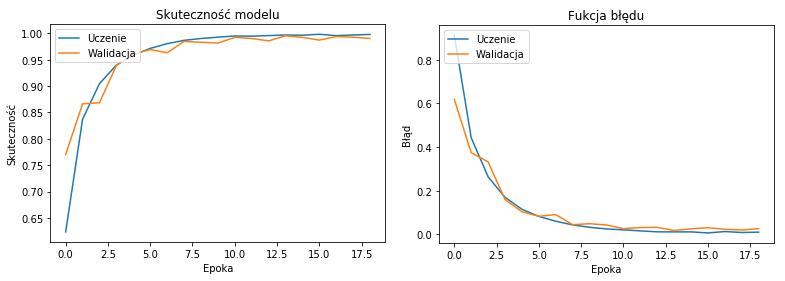
\includegraphics[scale=0.55]{VGG16_trainable_14_trening}	
	\caption{Zależność skuteczności i błędu od epoki trenowania modelu VGG16.}
	\label{fig:VGG16_trainable_14_trening}
\end{figure}

Sieć VGG została zbudowana w celu zwiększenia jakości klasyfikacji nie przez ilość warstw, ale przez wzrost liczby filtrów w poszczególnych warstwach. Wielkość filtrów jest stała i wynosi 3x3, są stosowane z krokiem jednego piksela. Użycie tak dużej ilości filtrów do stosunkowo małej bazy o czterech klasach w sytuacji, gdy wszystkie wagi modelu byłyby edytowalne, mógłby spowodować przetrenowanie zbioru. Z tego powodu w budowanej sieci zdecydowano się na zmniejszenie ilości filtrów do liczby dwucyfrowej w pojedynczej warstwie. Z sieci VGGNet zaczerpnięto logikę ułożenia typów warstw, gdyż po co dwóch lub trzech warstwach konwolucyjnych pojawia się warstwa redukcji maksymalizującej. Zastosowano też taką samą liczbę warstw redukcyjnych.

\begin{figure}[h!]
	\centering
	\centering
		\includegraphics[width=10cm,height=7cm]{U-Net_Structure}	
	\caption{Wizualizacja struktury sieci U-Net \cite{Silburt2019LunarCI}.}
	\label{fig:u-net_structure}
\end{figure}

}

\subsection{Cechy architektury zaczerpnięte z modelu U-Net.}

Architektura zaprezentowana w rozdziale \ref{sec:section_kaggle_1} wykazuje cechy struktury U-Net ze względu na kolejność ułożenia filtrów poszczególnej wielkości. Bazując na wiedzy, że użycie wspomnianej architektury dało wysokie rezultaty klasyfikacji, zastosowano podobne podejście. U-Net jest to sieć konwolucyjna opracowana na Uniwersytecie we Fryburgu do segmentacji obrazów biomedycznych \cite{Ronneberger2015UNetCN}. Typowa sieć U-Net nie ma w swojej strukturze warstw gęsto połączonych, a funkcją aktywacyjną jest zawsze ReLU. Opiera się na fakcie, że sieć neuronowa jest w stanie odfiltrować cechy ważne dla rozpoznania obiektów obrazu przez sukcesywne zmniejszanie wielkości filtrów, a potem ponowne zwiększanie do początkowej wielkości (Rys. \ref{fig:u-net_structure}). Zmniejszanie wymiaru następuje przez użcie warstw redukcyjnych, a zwiększanie przez konkatenację warstw. Jest to operacja podobna do działania filru dolnoprzepustowego, powodującego rozmycie obrazu, przez co traci się informację o szczegółach. Potem następuje ponowne odtworzenie danych w pierwotnej rozdzielczości na podstawie wygładzonego obrazu. Z architektury tej zaczerpnięto symetrię wielkości filtrów względem środkowej warstwy sieci.

\begin{figure}[h]
	\centering
	\centering
		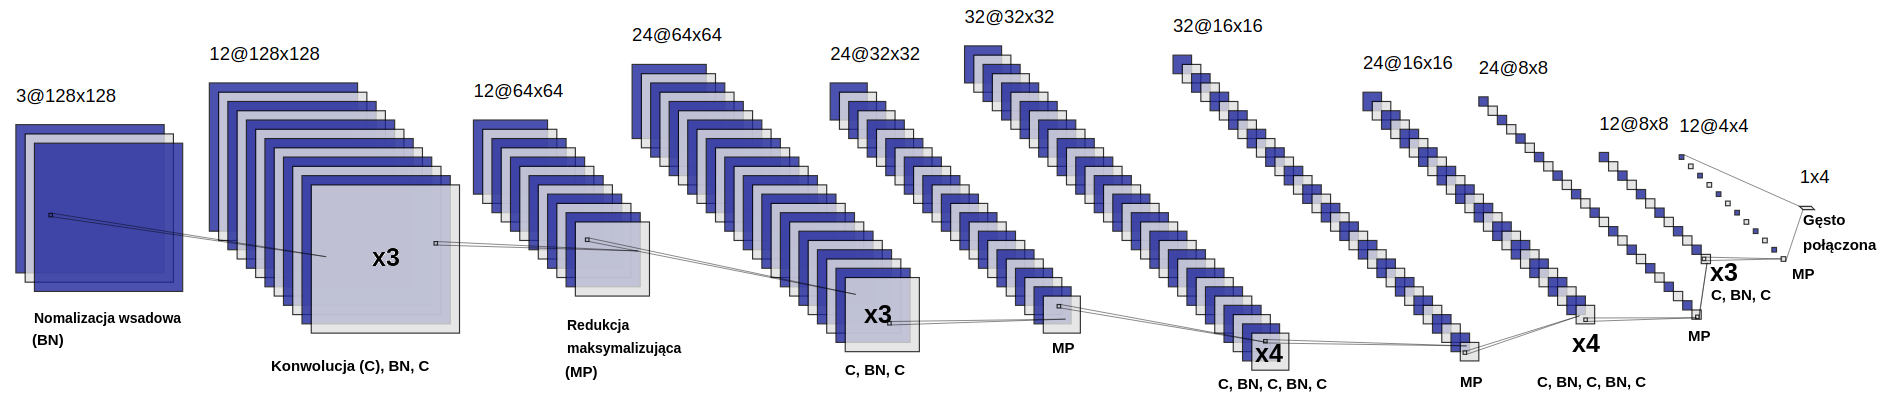
\includegraphics[scale=0.25]{my_model_structure_edited}	
	\caption{Wizualizacja struktury zaproponowanej sieci VGG-UNet.}
	\label{fig:vgg_unet_visualisation}
\end{figure}

{\parindent0pt
W żadnej ze wspomnianych architektur nie jest używana normalizacja wsadowa, zapewne dlatego, że zostały one opracowane zanim ten typ warstwy opisano i opublikowano w 2015 roku \cite{batch_normalisation}. W zaproponowanym modelu przed każdorazowym wejściem do warstwy konwolucyjnej są poddawane normalizacji. Jest to technika poprawiająca stabilność i jakość sieci neuronowych. Wyniki skuteczności klasyfikacji architektury z Rys. \ref{fig:vgg_unet_visualisation} są niższe niż sieci uprzednio przetrenowanej z powodu znacznie mniejszej sumarycznej liczby danych przepływających przez sieć w trakcie uczenia. Jednak fakt, że ponad połowa próbek została poprawnie zaklasyfikowana (\ref{tab:VGG_1_acc}) oraz nie ma klasy, która byłaby gorzej rozpoznawana niż inne (\ref{tab:VGG_1_params_val}) oznacza, że przy odpowiedniej edycji obecnego modelu można uzyskać wyższą skuteczność. Z wykresu treningu wynika, że opowiednia zmiana parametrów mogłaby pozwolić na wyższe osiągnięcia na zbiorze walidacyjnym, gdyż w obecnej postaci wyniki na tym zbiorze są mocno zaniżone (Rys. \ref{fig:VGG_1_trening}).

%VGG_1:
 \begin{table}[h!]
\centering
\caption[Short Heading]{Skuteczność modelu o strukturze VGG-UNet.}
\label{tab:VGG_1_acc}
\begin{tabular}{|c|c|c|c|}
\hline
\textbf{typ zbioru}           & \textbf{treningowy} & \textbf{walidacyjny} & \textbf{testowy} \\ \hline
\textbf{skuteczność {[}\%{]}} & 99                  & 64                   & 53               \\ \hline
\end{tabular}
\end{table}

\begin{table}[h!]
\centering
\caption[Short Heading]{Parametry mierzące jakość klasyfikacji na zbiorze testowym.}
\label{tab:VGG_1_params_val}
\begin{tabular}{|c|c|c|c|c|}
\hline
\textbf{Parametr}                               & \textbf{Precyzja} & \textbf{Czułość} & \textbf{Miara F1} & \textbf{Ilość próbek} \\ \hline
\textbf{klasa eozynofil (E)} & 0.26   & 0.29   & 0.27 & 623  \\ \hline
\textbf{klasa limfocyt (L)} & 0.24  & 0.23 & 0.23  & 620  \\ \hline
\textbf{klasa monocyt (M)} & 0.25   & 0.21    & 0.23  & 620  \\ \hline
\textbf{klasa neutrofil (N)} & 0.26   & 0.28    & 0.27  & 624  \\ \hline
\end{tabular}
\end{table}

\begin{figure}[h!]
	\centering
	\centering
		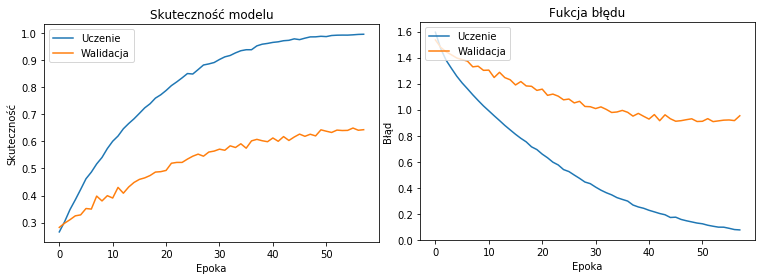
\includegraphics[scale=0.55]{VGG_1_trening}	
	\caption{Zależność skuteczności i błędu od epoki trenowania modelu o strukturze VGG-UNet.}
	\label{fig:VGG_1_trening}
\end{figure}
}

\subsection{Cechy architektury zaczerpnięte z modelu ResNet.}
\label{sec:architektura_resnet}

Warstwy w architekturze z rozdziału \ref{sec:section_kaggle_1} nie były połączone typowo sekwencyjnie. W co drugiej warstwie konwolucyjnej stosowano rozdzielenie sieci na dwie podsieci o takiej samej liczbie filtrów, ale różnej wielkości jądra. Wyjścia z tych warstw konkatenowano i wsadzano na kolejną warstwę konwolucyjną. Fragment struktury tej sieci obrazuje Rys. \ref{fig:struktura_modelu_231}. 


\begin{figure}[h!]
	\centering
	\centering
		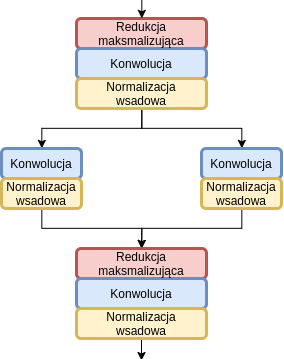
\includegraphics[width=7cm, height=7cm]{struktura_modelu_231}	
	\caption{Wizualizacja fragmentu struktury sieci z rozdziału \ref{sec:section_kaggle_1}.}	\label{fig:struktura_modelu_231}
\end{figure}

%ResNet_1
{\parindent0pt
Archiekturą, która także stosuje niesekwencyjne połączenie warstw jest rezydualna sieć (ang. \textit{residual neural network}, ResNet). Jej konstrukcja jest podobna do połączeń neuronów piramidowych w korze mózgowej. Wejścia w niej są połączone ze skonktenowanym wjściami warstwy bezpośrednio poprzedzającej oraz warstwy położonej kilka poziomów wcześniej \ref{fig:resnet_50}. W ten sposób omijane są połączenia z niektórymi warstwami. Najczęśćiej dotyczy to co drugiej lub co trzeciej warstwy. Pomijanie upraszcza sieć, co przyśpiesza proces uczenia. Inną korzyścią jest zmniejszenie problemu zanikajacych gradientów. Problem ten powstaje na etapie uczenia sieci korzystając z metod gradientowych. Poprawa wag w każdej iteracji jest proporcjnalna do pochodnej cząstkowej błędu funkcji względem obecnej wagi. Czasami może to prowadzić do sytuacji, gdzie gradient będzie tak mały, że waga nie zostanie zmieniona i postęp w nauce zostanie zatrzymany. Dzięki użyciu wag nie tylko z aktualnej warstwy, ale też z poprzedzającej \cite{vanishing_gradinets}. W przypadku modelu VGG-UNet nie używano funkcji aktywacyjnej mogącej spowodować zanikanie gradientu, gdyż aktywacją była funkcja ReLU. Mimo to po dołączeniu do modelu z Rys. \ref{fig:vgg_unet_visualisation}  połączenia typu ResNet, jak na Rys. \ref{fig:VGG_UNet_ResNet_structure}, wyniki na zbiorze testowym znacząco się poprawiły (\ref{tab:ResNet_1_acc}, \ref{tab:ResNet_1_params_val}). Z wykresów zależności skuteczności i błędu od epoki trenowania (\ref{fig:model_22_resnet_1_trening}) wynika, że klasyfikator należy dostroić, żeby zniwelować wahania wartości.

\begin{figure}[h!]
	\centering
	\centering
		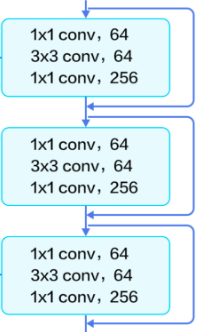
\includegraphics[scale=0.50]{resnet_50}	
	\caption{Wizualizacja fragmentu struktury sieci ResNet50 \cite{Res_Net_architecture}.}	\label{fig:resnet_50}
\end{figure}

\begin{figure}[h!]
	\centering
	\centering
		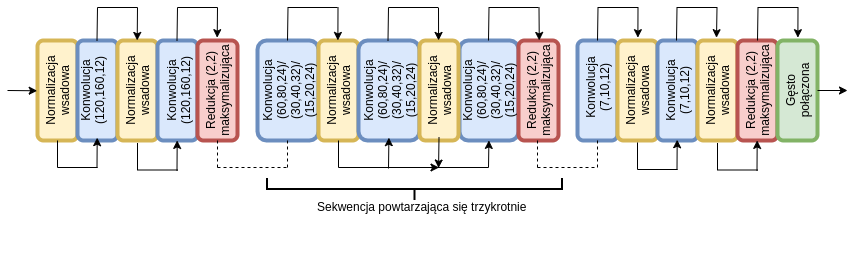
\includegraphics[scale=0.50]{VGG_UNet_ResNet_structure}	
	\caption{Wizualizacja architektury zaproponowanej sieci VGG-UNet-ResNet.}	\label{fig:VGG_UNet_ResNet_structure}
\end{figure}

\begin{table}[h!]
\centering
\caption[Short Heading]{Skuteczność modelu z cechami VGG-UNet-ResNet.}
\label{tab:ResNet_1_acc}
\begin{tabular}{|c|c|c|c|}
\hline
\textbf{typ zbioru}           & \textbf{treningowy} & \textbf{walidacyjny} & \textbf{testowy} \\ \hline
\textbf{skuteczność {[}\%{]}} & 99                  & 99                   & 86               \\ \hline
\end{tabular}
\end{table}

\begin{table}[h!]
\centering
\caption[Short Heading]{Parametry mierzące jakość klasyfikacji na zbiorze testowym modelu VGG-UNet-ResNet.}
\label{tab:ResNet_1_params_val}
\begin{tabular}{|c|c|c|c|c|}
\hline
\textbf{Parametr}                               & \textbf{Precyzja} & \textbf{Czułość} & \textbf{Miara F1} & \textbf{Ilość próbek} \\ \hline
\textbf{klasa eozynofil (E)} & 0.23   & 0.22   & 0.23 & 623  \\ \hline
\textbf{klasa limfocyt (L)} & 0.22  & 0.22 & 0.22 & 620  \\ \hline
\textbf{klasa monocyt (M)} & 0.24   & 0.18    & 0.21  & 620  \\ \hline
\textbf{klasa neutrofil (N)} & 0.24   & 0.31    & 0.27  & 624  \\ \hline
\end{tabular}
\end{table}

\begin{figure}[h!]
	\centering
	\centering
		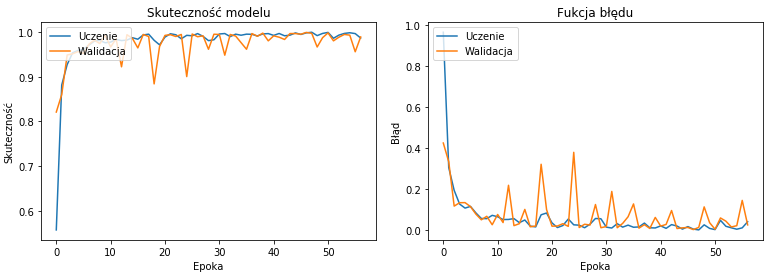
\includegraphics[scale=0.50]{model_22_resnet_1_trening}	
	\caption{Zależność skuteczności i błędu od epoki trenowania modelu o strukturze VGG-UNet-ResNet.}	\label{fig:model_22_resnet_1_trening}
\end{figure}

}
\section{Dobór parametrów}
\label{dobor_parametrow}

Podczas uczenia zaproponowanego modelu widoczne są duże wahania skuteczności i błędu na zbiorze walidacyjnym (\ref{fig:model_22_resnet_1_trening}). Jest to dowód na nadmierne dopasowanie, gdyż wykres opisuje w dużej części szum. Może to być spowodowane słabym dobraniem modelu do zadania i oznacza konieczność dostrojenia parametrów. Jeśli mimo prób doboru parametrów krzywa walidayjna nadal będzie zaszumiona, możliwe że baza danych musi zostać podzielona raz jeszcze, gdyż zbiór walidacyjny jest niereprezentacyjny \cite{learning_curve_diagnostics}.

{\parindent0pt
Strojenie parametrów wykonuje się w celu uzyskania jak najszybszej zbieżności modelu do wyniku, więc im mniej epok zajmuje trening tym lepsza jest opracowna sieć. Jednocześnie należy przy tym zachować wysoką precyzję rozwiązania, która jest mierzona przez skuteczność klasyfikacji. Innym ważnym aspektem, jaki należy wziąć pod uwagę jest złożoność obliczeniowa, jeśli klasyfikator posiada wiele warstw i filtrów, to jego użycie będzie zajmowało dużo mocy obliczeniowej. Należy dążyć do jak prostej struktury, która będzie dawała dobre efekty. W tym celu zostanie przetestowanych kilka wariantów wybranych parametrów modelu, a wyniki porównane z uzyskanymi w rozdziale \ref{sec:architektura_resnet}. Końcowy model zostanie zaprezentowany w rozdziale \ref{cha:analiza_wynikow}, gdzie zamieszczona zostanie analiza wyników klasyfikacji.
}
\subsection{Dobór optymalizatora i szybkości uczenia}

Jednym z powodów wahań skuteczności modelu na przestrzenii epok może być niepoprawnie dobrany krok w minimalizacji funkcji błędu. W pierwszym podejściu używany był optymalizator ADAM (\ref{equ:adam}) z krokiem równym \num{1e-3}. Jest to metoda optymalizacji bazująca na RMSprop (\ref{equ:rmsprop}), z użyciem dodatkowo stochastycznego spadku gradientowego z bezwładnością. Istnieją różne warjancje optymalizator ADAM, w tym NADAM, gdzie bezwładność liczona jest algorytmem Nesterova. Wykonano serię eksperymentów używając optymalizatorów: RMSprop, Adam i Nadam oraz różnej wielkości kroku. Dla wszystkich typów badanych optymalizatorów najlepsza wielkość kroku to \num{2e-4}. Poniżej przedstawiono porównanie optymalizatorów z tym krokiem.

\begin{figure}[h!]
	\centering
	\centering
		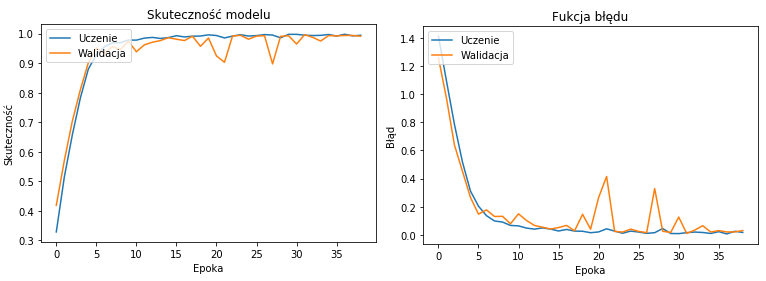
\includegraphics[scale=0.50]{opt_Nadam_4_trening}	
	\caption{Zależność skuteczności i błędu od epoki trenowania dla optymalizatora NADAM z krokiem \num{2e-4}.}	\label{fig:opt_Nadam_4_trening}
\end{figure}

\begin{figure}[h!]
	\centering
	\centering
		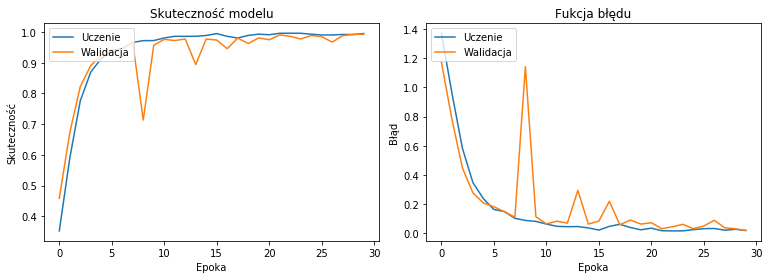
\includegraphics[scale=0.50]{opt_Adam_4_trening}	
	\caption{Zależność skuteczności i błędu od epoki trenowania dla optymalizatora ADAM z krokiem \num{2e-4}.}	\label{fig:opt_Adam_4_trening}
\end{figure}

\begin{figure}[h!]
	\centering
	\centering
		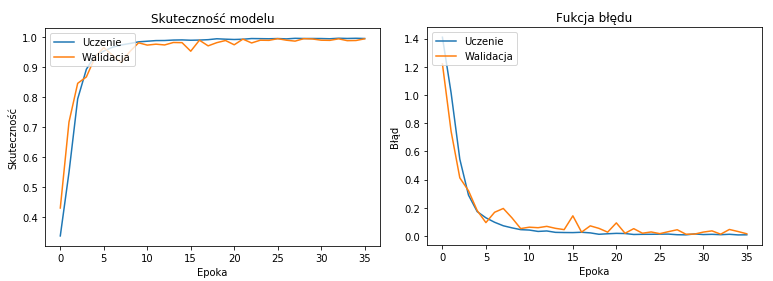
\includegraphics[scale=0.50]{opt_RMSprop_trening}	
	\caption{Zależność skuteczności i błędu od epoki trenowania dla optymalizatora RMSprop z krokiem \num{2e-4}.}	\label{fig:opt_RMSprop_trening}
\end{figure}
{\parindent0pt
W przypadku algorytmu NADAM (\ref{fig:opt_Nadam_4_trening}) wahania są rzadsze niż przy użyciu oryginalnego optymalizatora (\ref{fig:model_22_resnet_1_trening}), jednak wykres nie wykazuje tendencji do stabilizacji. Uczenie z użyciem optymalizatora ADAM wykazuje pozytywną cechę zanikania wahań (\ref{fig:opt_Adam_4_trening}), więc wybór tego wariantu miałby sens. Jednak najmniejsze wahania i tendencję do ich wygłuszania można zaobserwować na wykresie optymalizatora RMSprop (\ref{fig:opt_RMSprop_trening}). Z tego powodu kolejne eksperymenty będą przeprowadzane z użyciem RMSprop i kroku \num{2e-4}.
}

\subsection{Ograniczenie przeuczenia modelu}
CNN są sieciami posiadającymi poza warstwami konwolucyjnymi i redukcyjnymi warstwy w pełni połączone (ang. \textit{fully-connected network}). Charakteryzują się one tym, że każdy neuron posiada połączenie z dowolnym innym neuronem w poprzedniej warstwie. To sprawia, że są podatne na zjawisko nadmiernego dopasowania. 

{\parindent0pt
Jednym ze sposobów na uniknięcie nadmiernego dopasowania jest używanie warstw regularyzacyjnych, takich jak normalizacja wsadowa. Oryginalnie w architekturach VGG16, U-Net i ResNet tego typu warstwa nie jest używana. Mimo to, w zaproponowanym modelu zdecydowano się na jej użycie, gdyż pozwala to na o wiele lepsze wyniki w porównaniu do sieci bez tej warstwy (\ref{fig:model_32_resnet_1_noBN_trening}).

\begin{figure}[h!]
	\centering
	\centering
		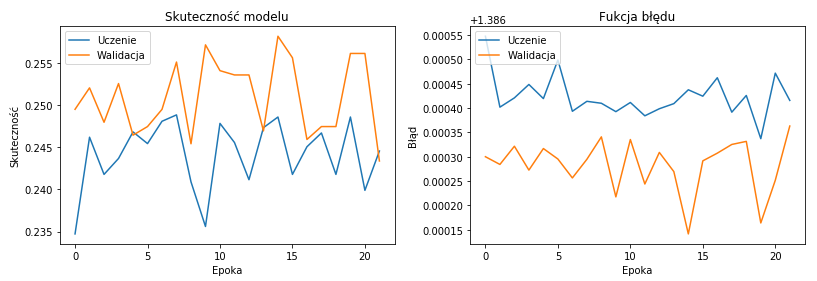
\includegraphics[scale=0.50]{model_32_resnet_1_noBN_trening}	
	\caption{Zależność skuteczności i błędu od epoki trenowania modelu o strukturze VGG-UNet-ResNet bez warstw normalizacji wsadowej.}	\label{fig:model_32_resnet_1_noBN_trening}
\end{figure}

Innym sposobem, poza użyciem konkretnych warstw, jest przeprowadzenie treningu w taki sposób, aby nie dopuścić do przeuczenia modelu. W tym celu w każdej epoce nauki należy monitorować wartość błędu na zbiorze walidacyjnym i porównywać z błędem w poprzedniej epoce. Jeśli nie obserwuje się poprawy przez daną ilość epok, w omawianym modelu ta wartość wynosi 7, to trening zostaje przerwany. Ma to na celu zachowanie ogólności działania klasyfikatora i uniknięcie takiego ustawienia wag, aby model dopasował się jedynie do konkretnych danych w zbiorze uczącym. 
%https://en.wikipedia.org/wiki/Early_stopping
}

\subsection{Wpływ przygotowania danych na jakość klasyfikacji}

Oryginalnie dane przed przejściem przez sieć neuronową są normalizowane zgodnie z rozdziałem \ref{przygotowanie_danych}. Wykonano eksperyment, w którym pominięto krok normalizacji danych. Wyniki i jakość modelu nie uległy znacznemu pogorszeniu (\ref{fig:no_rescale_rgb_12_24_32_trening}), z powodu użycia warstwy normalizacji wsadowej na początku sieci neuronowej. Kształt wejścia do modelu zachowano bez zmian: 120x160x3. Skuteczność na zbiorze walidacyjnym i treningowym wynosiła nadal 99\%.

\begin{figure}[h!]
	\centering
	\centering
		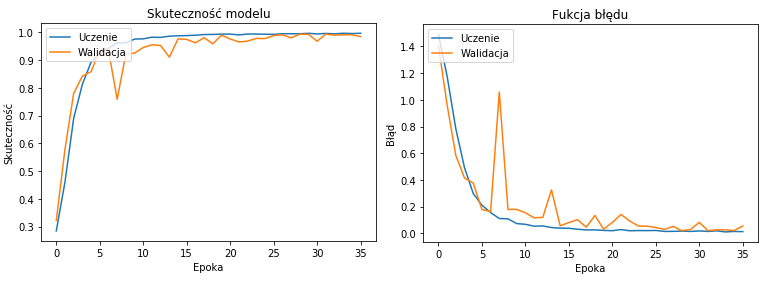
\includegraphics[scale=0.50]{no_rescale_rgb_12_24_32_trening}	
	\caption{Zależność skuteczności i błędu od epoki trenowania modelu przetrenowanego na ramkach RGB nie znormalizowanych.}	\label{fig:no_rescale_rgb_12_24_32_trening}
\end{figure}

{\parindent0pt
W kolejnym eksperymencie także nie wykonano normalizacji, a dodatkowo zmniejszono liczbę kanałów do jednego, czyli spłycono ilość informacji do jasności pikseli. Nie tylko pogorszyło to jakość procesu uczenia, ale też obniżyło skuteczność na zbiorze walidacyjnym o dwa punkty procentowe \ref{fig:no_rescale_grayscale_12_24_32_trening}).

\begin{figure}[h!]
	\centering
	\centering
		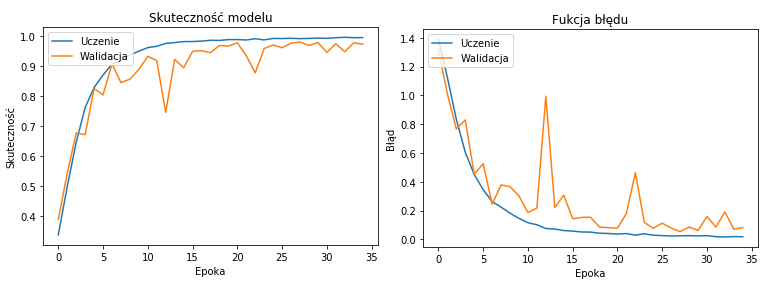
\includegraphics[scale=0.50]{no_rescale_grayscale_12_24_32_trening}	
	\caption{Zależność skuteczności i błędu od epoki trenowania modelu przetrenowanego na ramkach Grayscale, nie znormalizowanych.}	\label{fig:no_rescale_grayscale_12_24_32_trening}
\end{figure}

Dane wprowadzane do sieci neuronowej są dzielone na porcje (ang. \textit{batches}), co odciąża maszynę liczącą i pozwala na przyspieszenie procesu uczenia. Każdy podzbiór: uczący, walidacyjny i testowy dzielony jest na porcje o tej samej liczebności. Początkowym podejściem był podział na porcje o zawartości 32 elementów. Typowo sieci uczą się szybciej na porcjach o małej liczebności oraz zbiegają do płaskich minimów (\ref{fig:sharp_flat_min}) . Z kolei przy stosowaniu dużej liczbeności obserwuje się degradację jakości modelu, w szczególności dotyczącej zdolności do generalizacji. Jest to spowodowane tendencją do zbieżności tego typu algorytmów do ostrych minimów, która nie sprzyja generalizacji rozwiązania \cite{Keskar2016OnLT}. 

\begin{figure}[h!]
	\centering
	\centering
		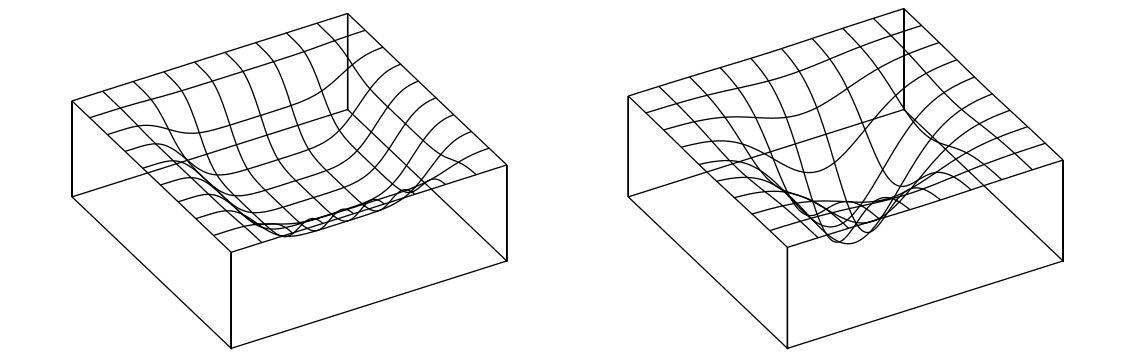
\includegraphics[scale=0.50]{sharp_flat_min}	
	\caption{Wizualizacja różnicy między minimum płaskim (z lewej), a ostrym (z prawej) \cite{sharp_flat_min}.}	\label{fig:sharp_flat_min}
\end{figure}

W niektórych przypadkach powiększenie batchy ma pozytywy wpływ. Na przykład dla sieci AlexNet uczonej na obrazach ImageNet zwiększenie liczebności z 512 do 4096 poskutkowało trzykrotnym przyśpieszeniem procesu uczenia \cite{You2017ScalingSB}. W przypadku omawianego modelu podział na porcje o większej liczebności niż 32 skutkuje niedouczeniem sieci (ang. \textit{underfitting}), zarówno dla 128 jak i 512 ramek (\ref{fig:128_batch_12_24_32_trening}, \ref{fig:512_batch_12_24_32_trening}). Dla liczebności miejszej niż 32 też występuje taki sam problem (\ref{fig:16_batch_12_24_32_trening}). Na tej podstawie można wnioskować, że wybór 32 ramek w porcji jest najlepszym podziałem.

\begin{figure}[H]
	\centering
	\centering
		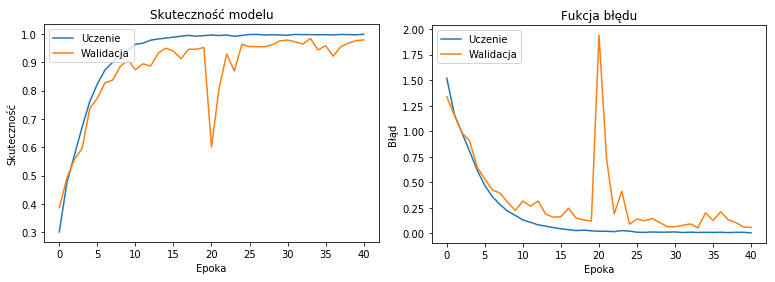
\includegraphics[scale=0.50]{128_batch_12_24_32_trening}	
	\caption{Zależność skuteczności i błędu od epoki modelu trenowanego z użyciem bazy podzielonej na batche o liczebności 128 ramkek.}	\label{fig:128_batch_12_24_32_trening}
\end{figure}

\begin{figure}[H]
	\centering
	\centering
		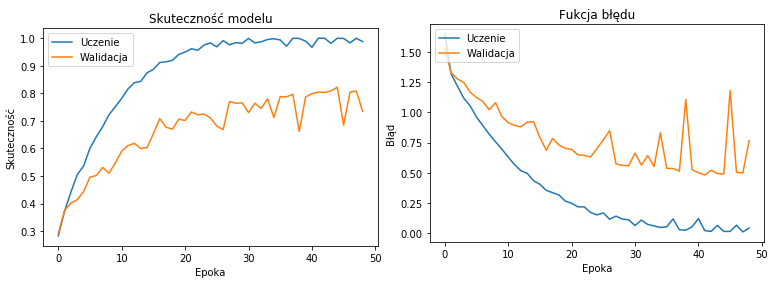
\includegraphics[scale=0.50]{512_batch_12_24_32_trening}	
	\caption{Zależność skuteczności i błędu od epoki modelu trenowanego z użyciem bazy podzielonej na batche o liczebności 512 ramkek.}	\label{fig:512_batch_12_24_32_trening}
\end{figure}

\begin{figure}[H]
	\centering
	\centering
		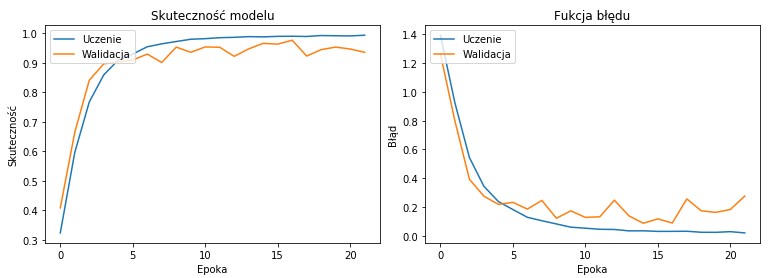
\includegraphics[scale=0.50]{16_batch_12_24_32_trening}	
	\caption{Zależność skuteczności i błędu od epoki modelu trenowanego z użyciem bazy podzielonej na batche o liczebności 16 ramkek.}	\label{fig:16_batch_12_24_32_trening}
\end{figure}
}

\subsection{Wybór funkcji redukcyjnej}

Dotychczas stosowanym typem warstwy redukcyjnej była maksymalizacja o oknie wielkości 2x2 stosowana z krokiem dwóch pikseli. Oznacza to, że wybiera ona najjaśniejsze piksele z obrazu. Jest więc przydatna do klasyfikacji obiektów jasnych na ciemniejszym od nich tle. W eksperymencie sprawdzono jaki wpływ na przebieg uczenia będzie miało zamienienie wszystkich warstw reducyjnych na minimalizację lub średnią arytmetyczną, także o wielkości 2x2. 

\begin{figure}[H]
	\centering
	\centering
		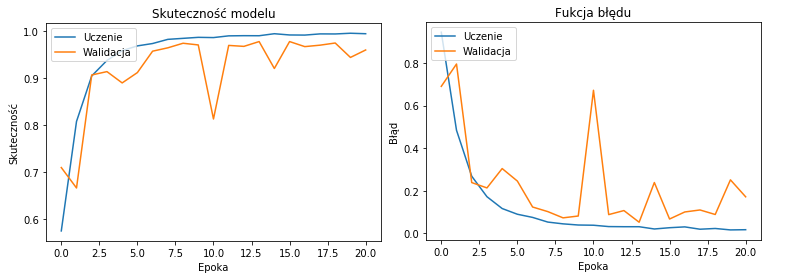
\includegraphics[scale=0.50]{filters_12_24_32_AP_trening}	
	\caption{Zależność skuteczności i błędu od epoki modelu trenowanego z użyciem warstw redukcji uśredniającej.}	\label{fig:filters_12_24_32_AP_trening}
\end{figure}

\begin{figure}[H]
	\centering
	\centering
		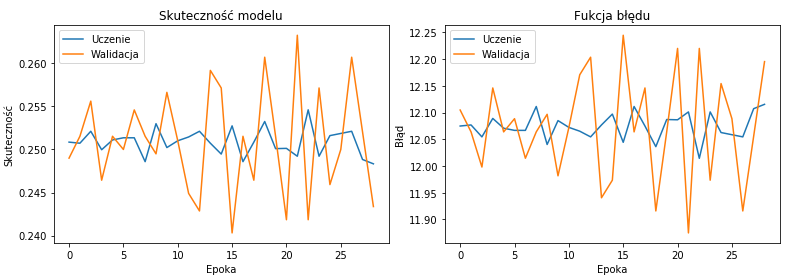
\includegraphics[scale=0.50]{filters_12_24_32_minpooling_trening}	
	\caption{Zależność skuteczności i błędu od epoki modelu trenowanego z użyciem warstw redukcji uśredniającej.}	\label{fig:filters_12_24_32_minpooling_trening}
\end{figure}

{\parindent0pt
Użycie średniej arytmetycznej jedynie nieznacznie zabrzyło proces, powodując wahania skuteczności wlidacyjnej i niedotrenowanie (\ref{fig:filters_12_24_32_AP_trening}). Skuteczność na zbiorze walidacyjnym spadła, ale nie drastycznie. Powodem takiego zachowania jest fakt, że redukcja uśredniająca wygładza obraz i powoduje, że detale mogą zostać pominięte. Ramki są nadal klasyfikowane poprawnie, ale w mniejszej ilości niż miało to miejsce w przypadku redukcji aksymalizujące. Z kolei warstwy minimalizacyjne całkowicie zablokowały proces uczenia, który zatrzymał się w minimum lokalnym dającym około 25\% skuteczności. Filtr typu min podkreśla ciemne piksele. Sprawia to, że krwinki nie mające jądra, widoczne w tle zdjęcia stają się bardziej wyraźne (\ref{fig:reduction_layers}). Zaciemnia to obraz i sprawia, że rozpoznanie typu krwinki staje się trudniejsze. Ponadto jądro, które jest ciemne na tle reszty krwinki zostaje powiększone we wszystkich typach krwinek (\ref{fig:neutrofil_reduction_layers}), przez to algorytm myli jądra dwupłatowe i posegmentowane z jądrami kulistymi i klasyfikuje wszystkie typy krwinek jako neutrofil (\ref{tab:min_red_layers_params_val}). Ramki, które zostały poddane działaniu filtru maksymalizującego zachowują bardziej czytelną informację dotyczącą typu jądra, co szczególnie jest widoczne w jądrach niekulistych (\ref{fig:neutrofil_reduction_layers}).

\begin{figure}[h!]
	\centering
	\centering
		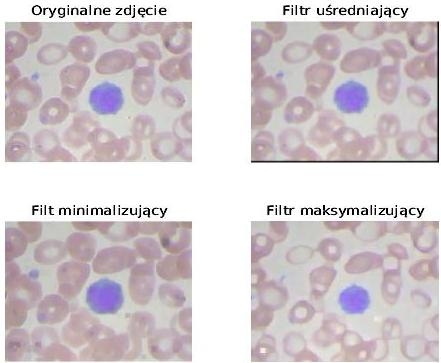
\includegraphics[scale=0.7]{reduction_layers}	
	\caption{Zdjęcie limfocytu z bazy po pięciokrotnym nałożeniu filtrów 2x2.}	\label{fig:reduction_layers}
\end{figure}

\begin{figure}[h!]
	\centering
	\centering
		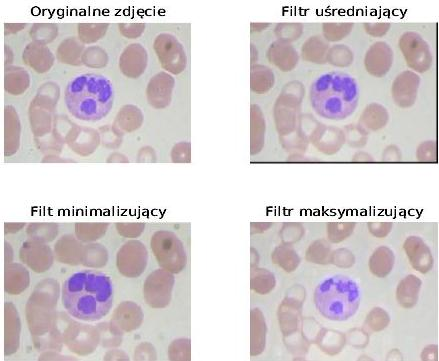
\includegraphics[scale=0.7]{neutrofil_reduction_layers}	
	\caption{Zdjęcie neutrofilu z bazy po pięciokrotnym nałożeniu filtrów 2x2.}\label{fig:neutrofil_reduction_layers}
\end{figure}

\begin{table}[h!]
\centering
\caption[Short Heading]{Parametry mierzące jakość klasyfikacji na zbiorze walidacyjnym modelu z warstwą redukcyjną minimalizującą.}
\label{tab:min_red_layers_params_val}
\begin{tabular}{|c|c|c|c|c|}
\hline
\textbf{Parametr}                               & \textbf{Precyzja} & \textbf{Czułość} & \textbf{Miara F1} & \textbf{Ilość próbek} \\ \hline
\textbf{klasa eozynofil (E)} & 0.00   & 0.00   & 0.00 & 499  \\ \hline
\textbf{klasa limfocyt (L)}& 0.00   & 0.00   & 0.00 & 497  \\ \hline
\textbf{klasa monocyt (M)} & 0.00   & 0.00   & 0.00 & 496  \\ \hline
\textbf{klasa neutrofil (N)} & 0.25   & 1.00    & 0.40  & 500  \\ \hline
\end{tabular}
\end{table}
}

\subsection{Wybór funkcji aktywacyjnej warstw konwolucyjnych}

W modelu użytą funkcją aktywacyjną dla wszystkich warstw konwolucyjnych jest ReLU (\ref{equ:activ_relu}). W celu dobrania optymalnej aktwacji sprawdzono działanie sieci także dla aktywacji liniowej (\ref{equ:activ_linear}) z współczynnikiem c = 1, eksponencjalnej (\ref{equ:activ_exp}) i tangensa hiperbolicznego (\ref{equ:activ_tanh}). 

\begin{figure}[h!]
	\centering
	\centering
		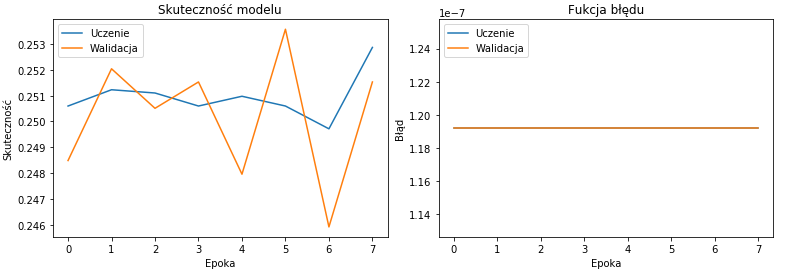
\includegraphics[scale=0.5]{filters_12_24_32_exp_trening}	
	\caption{Zależność skuteczności i błędu od epoki modelu trenowanego z użyciem aktywacji eksponencjalnej w warstwach konwolucyjnych.}\label{fig:filters_12_24_32_exp_trening}
\end{figure}

\begin{table}[h!]
\centering
\caption[Short Heading]{Parametry mierzące jakość klasyfikacji na zbiorze walidacyjnym modelu z warstwą aktywacyjną eksponencjalną.}
\label{tab:exp_act_layers_params_val}
\begin{tabular}{|c|c|c|c|c|}
\hline
\textbf{Parametr}                               & \textbf{Precyzja} & \textbf{Czułość} & \textbf{Miara F1} & \textbf{Ilość próbek} \\ \hline
\textbf{klasa eozynofil (E)} & 0.25   & 1.00   & 0.40 & 499  \\ \hline
\textbf{klasa limfocyt (L)}& 0.00   & 0.00   & 0.00 & 497  \\ \hline
\textbf{klasa monocyt (M)} & 0.00   & 0.00   & 0.00 & 496  \\ \hline
\textbf{klasa neutrofil (N)} & 0.00   & 0.00    & 0.00  & 500  \\ \hline
\end{tabular}
\end{table}

{\parindent0pt
Najmniej zadowalające wyniki dało użycie funkcji eksponencjalnej, gdyż algorytm utyka w minimum lokalnym już w pierwszej epoce i rozpoznawaje poprawnie jedynie klasę eozynofil. Zmiana wielkości kroku przy poszukiwaniu minimum nie przyniosła pozytywnych rezultatów. Zmiany wag w kolejnych epokach nie skutkowały zmianą wartości funkcji błędu (\ref{fig:filters_12_24_32_exp_trening}). Parametry macierzy pomyłek zbioru wlidacyjnego wskazują na to, że aktywacja eksponencjalna prowadzi do przyporządkowania zawsze tej samej wartości wyjściowej niezależnie od wejścia (\ref{tab:exp_act_layers_params_val}).

\begin{figure}[h!]
	\centering
	\centering
		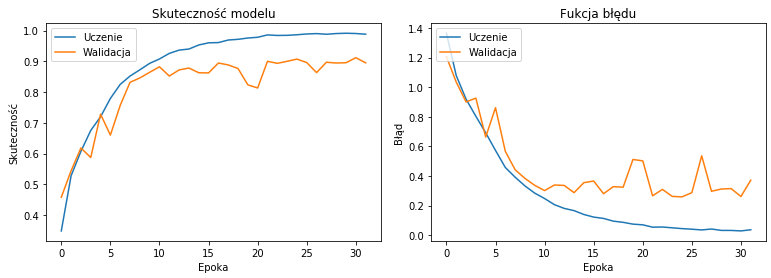
\includegraphics[scale=0.5]{filters_12_24_32_linear_trening}	
	\caption{Zależność skuteczności i błędu od epoki modelu trenowanego z użyciem aktywacji liniowej w warstwach konwolucyjnych.}\label{fig:filters_12_24_32_linear_trening}
\end{figure}

\begin{table}[h!]
\centering
\caption[Short Heading]{Parametry mierzące jakość klasyfikacji na zbiorze walidacyjnym modelu z warstwą aktywacyjną liniową.}
\label{tab:lin_act_layers_params_val}
\begin{tabular}{|c|c|c|c|c|}
\hline
\textbf{Parametr}                               & \textbf{Precyzja} & \textbf{Czułość} & \textbf{Miara F1} & \textbf{Ilość próbek} \\ \hline
\textbf{klasa eozynofil (E)} & 0.25   & 0.22   & 0.24 & 499  \\ \hline
\textbf{klasa limfocyt (L)}& 0.21   & 0.20   & 0.21 & 497  \\ \hline
\textbf{klasa monocyt (M)} & 0.23   & 0.24   & 0.24 & 496  \\ \hline
\textbf{klasa neutrofil (N)} & 0.25   & 0.27    & 0.26 & 500  \\ \hline
\end{tabular}
\end{table}

Lepszą jakość klasyfikacji uzyskano przy użyciu jednej z najprostszych aktywacji - liniowej. W tym typie aktywacji wartość na wejściu jest przekazywana bezpośrednio na wyjście, gdyż współczynnik skalowania wynosi 1. Model rozpoznaje poprawnie pewną ilość danych z każdej klasy, jednak w porównaniu z aktywacją ReLU radzi sobie gorzej (\ref{tab:lin_act_layers_params_val}). W procesie uczenia można zaobserwować underfitting (\ref{fig:filters_12_24_32_linear_trening}). Wybrany typ aktywacji nie odwzorowuje skomplikowanych typów funkcji i nie wprowadza elementów nieliniowych do modelu, co jest głównym celem użycia aktywacji. Z pewnością ten klasyfikator ma niższą złożoność obliczeniową, ale jest ograniczony w zakresie skomplikowania funkcji, których jest w stanie się nauczyć. Przez to jest słabszym narzędziem i jego działanie podobne jest do działania liniowych modeli regresji. Nie spełnia on więc odpowiednio swojej funkcji w sieci głębokiej.

\begin{figure}[h!]
	\centering
	\centering
		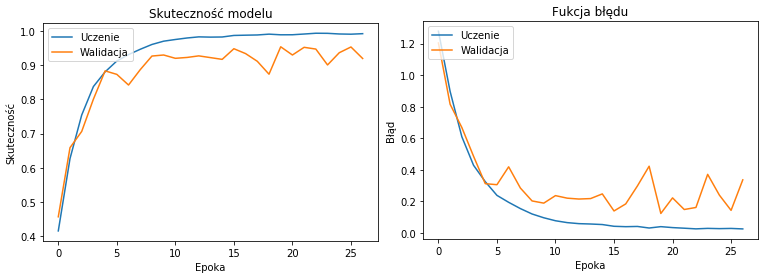
\includegraphics[scale=0.5]{filters_12_24_32_tanh_trening}	
	\caption{Zależność skuteczności i błędu od epoki modelu trenowanego z użyciem aktywacji tangensa hiperbolicznego w warstwach konwolucyjnych.}\label{fig:filters_12_24_32_tanh_trening}
\end{figure}

\begin{table}[h!]
\centering
\caption[Short Heading]{Parametry mierzące jakość klasyfikacji na zbiorze walidacyjnym modelu z warstwą aktywacyjną tangensa hiperbolicznego.}
\label{tab:tanh_act_layers_params_val}
\begin{tabular}{|c|c|c|c|c|}
\hline
\textbf{Parametr}                               & \textbf{Precyzja} & \textbf{Czułość} & \textbf{Miara F1} & \textbf{Ilość próbek} \\ \hline
\textbf{klasa eozynofil (E)} & 0.26   & 0.22   & 0.24 & 499  \\ \hline
\textbf{klasa limfocyt (L)}& 0.26   & 0.27   & 0.26 & 497  \\ \hline
\textbf{klasa monocyt (M)} & 0.25   & 0.24   & 0.25 & 496  \\ \hline
\textbf{klasa neutrofil (N)} & 0.26   & 0.29    & 0.27 & 500  \\ \hline
\end{tabular}
\end{table}

Aktywacja z użyciem tangensa hiperbolicznego dała jeszcze lepsze efekty. Mimo, że nadal w tej wersji występuje duże niedotrenowanie (\ref{fig:filters_12_24_32_tanh_trening}), to precyzja klasyfikacji na zbiorze walidacyjnym wzrosła w porównaniu do aktywacji liniowej (\ref{tab:tanh_act_layers_params_val}). Tangens hiperboliczny jest narażony na występowanie zjawiska zanikania gradientu, dlatego zaleca się stosowanie aktywacji ReLU \cite{activation_functions}. Z teo powodu, że żadna z aktywacji nie dała lepszych rezultatów niż pierwotne podejście funkcją aktywacyjną pozostaje ReLU (\ref{fig:opt_RMSprop_trening}).

}

%\subsection{Dostosowanie parametrów filtrów - nie wiem czy jest sens bo wychodzi tak samo wszystko}

%W oryginalnej strukturze modelu zastosowano sekwencję rozmiaru filtrów inspirowaną architekturą U-Net, gdyż inne podejścia nie były efektowne. Po nastrojeniu optymalizatora ponownie przebadano różnego typu układy filtrów.

%wielkość: -nie wiem, może po doborze optymalizatora będzie jakaś różnica - póki co wszystko jedno. Max acc dla 12-18-24 i 12-24-36, czyli nie ma zasady, pewnie losowe.

%padding: tutaj tylko 2 opcje do sprawdzenia

%wielkość kernela: jak nie zmienisz znacząco to nie zobaczysz różnicy, nie wiem czy jest sens testować - na potem


%teraz sposoby jak sobie z tym radzić poza augmentation
%coś o regularyzacji: https://towardsdatascience.com/training-deep-neural-networks-9fdb1964b964, dorzuć podobny obrazek do overfittingu żeby było wiadomo co to
%oraz o bach normalisation: https://towardsdatascience.com/batch-normalization-in-neural-networks-1ac91516821c
